%%%%%%%%%%%%%%%%%%%%%%%%%%%%%%%%%%%%%%%%%
% Jacobs Landscape Poster
% LaTeX Template
% Version 1.1 (14/06/14)
%
% Created by:
% Computational Physics and Biophysics Group, Jacobs University
% https://teamwork.jacobs-university.de:8443/confluence/display/CoPandBiG/LaTeX+Poster
% 
% Further modified by:
% Nathaniel Johnston (nathaniel@njohnston.ca)
%
% This template has been downloaded from:
% http://www.LaTeXTemplates.com
%
% License:
% CC BY-NC-SA 3.0 (http://creativecommons.org/licenses/by-nc-sa/3.0/)
%
%%%%%%%%%%%%%%%%%%%%%%%%%%%%%%%%%%%%%%%%%

%----------------------------------------------------------------------------------------
%	PACKAGES AND OTHER DOCUMENT CONFIGURATIONS
%----------------------------------------------------------------------------------------

\documentclass[final]{beamer}

\usepackage[scale=1.0]{beamerposter} % Use the beamerposter package for laying out the poster
\usepackage[acronym,toc]{glossaries}
\newacronym[longplural={metric tons of heavy metal}]{MTHM}{MTHM}{metric ton of heavy metal}
\newacronym{ABM}{ABM}{agent-based modeling}
\newacronym{ACDIS}{ACDIS}{Program in Arms Control \& Domestic and International Security}
\newacronym{AHTR}{AHTR}{Advanced High Temperature Reactor}
\newacronym{ANDRA}{ANDRA}{Agence Nationale pour la gestion des D\'echets RAdioactifs, the French National Agency for Radioactive Waste Management}
\newacronym{ANL}{ANL}{Argonne National Laboratory}
\newacronym{API}{API}{application programming interface}
\newacronym{ARCH}{ARCH}{autoregressive conditional heteroskedastic}
\newacronym{ARE}{ARE}{Aircraft Reactor Experiment}
\newacronym{ARFC}{ARFC}{Advanced Reactors and Fuel Cycles}
\newacronym{ARMA}{ARMA}{autoregressive moving average}
\newacronym{ASME}{ASME}{American Society of Mechanical Engineers}
\newacronym{ATWS}{ATWS}{Anticipated Transient Without Scram}
\newacronym{BDBE}{BDBE}{Beyond Design Basis Event}
\newacronym{BIDS}{BIDS}{Berkeley Institute for Data Science}
\newacronym{BOL}{BOL}{Beginning-of-Life}
\newacronym{BSD}{BSD}{Berkeley Software Distribution}
\newacronym{CAFCA}{CAFCA}{ Code for Advanced Fuel Cycles Assessment }
\newacronym{CASL}{CASL}{Consortium for Advanced Simulation of Light Water Reactors}
\newacronym{CDTN}{CDTN}{Centro de Desenvolvimento da Tecnologia Nuclear}
\newacronym{CEA}{CEA}{Commissariat \`a l'\'Energie Atomique et aux \'Energies Alternatives}
\newacronym{CI}{CI}{continuous integration}
\newacronym{CNEC}{CNEC}{Consortium for Nonproliferation Enabling Capabilities}
\newacronym{CNEN}{CNEN}{Comiss\~{a}o Nacional de Energia Nuclear}
\newacronym{CNERG}{CNERG}{Computational Nuclear Engineering Research Group}
\newacronym{COSI}{COSI}{Commelini-Sicard}
\newacronym{COTS}{COTS}{commercial, off-the-shelf}
\newacronym{CSNF}{CSNF}{commercial spent nuclear fuel}
\newacronym{CTAH}{CTAHs}{Coiled Tube Air Heaters}
\newacronym{CUBIT}{CUBIT}{CUBIT Geometry and Mesh Generation Toolkit}
\newacronym{CURIE}{CURIE}{Centralized Used Fuel Resource for Information Exchange}
\newacronym{DAG}{DAG}{directed acyclic graph}
\newacronym{DANESS}{DANESS}{Dynamic Analysis of Nuclear Energy System Strategies}
\newacronym{DBE}{DBE}{Design Basis Event}
\newacronym{DESAE}{DESAE}{Dynamic Analysis of Nuclear Energy Systems Strategies}
\newacronym{DHS}{DHS}{Department of Homeland Security}
\newacronym{DOE}{DOE}{Department of Energy}
\newacronym{DRACS}{DRACS}{Direct Reactor Auxiliary Cooling System}
\newacronym{DRE}{DRE}{dynamic resource exchange}
\newacronym{DSNF}{DSNF}{DOE spent nuclear fuel}
\newacronym{DYMOND}{DYMOND}{Dynamic Model of Nuclear Development }
\newacronym{EBS}{EBS}{Engineered Barrier System}
\newacronym{EDZ}{EDZ}{Excavation Disturbed Zone}
\newacronym{EIA}{EIA}{U.S. Energy Information Administration}
\newacronym{EPA}{EPA}{Environmental Protection Agency}
\newacronym{EP}{EP}{Engineering Physics}
\newacronym{FCO}{FCO}{Fuel Cycle Options}
\newacronym{FCT}{FCT}{Fuel Cycle Technology}
\newacronym{FCWMD}{FCWMD}{Fuel Cycle and Waste Management Division}
\newacronym{FEHM}{FEHM}{Finite Element Heat and Mass Transfer}
\newacronym{FEPs}{FEPs}{Features, Events, and Processes}
\newacronym{FHR}{FHR}{Fluoride-Salt-Cooled High-Temperature Reactor}
\newacronym{FLiBe}{FLiBe}{Fluoride-Lithium-Beryllium}
\newacronym{GCAM}{GCAM}{Global Change Assessment Model}
\newacronym{GDSE}{GDSE}{Generic Disposal System Environment}
\newacronym{GDSM}{GDSM}{Generic Disposal System Model}
\newacronym{GENIUSv1}{GENIUSv1}{Global Evaluation of Nuclear Infrastructure Utilization Scenarios, Version 1}
\newacronym{GENIUSv2}{GENIUSv2}{Global Evaluation of Nuclear Infrastructure Utilization Scenarios, Version 2}
\newacronym{GENIUS}{GENIUS}{Global Evaluation of Nuclear Infrastructure Utilization Scenarios}
\newacronym{GPAM}{GPAM}{Generic Performance Assessment Model}
\newacronym{GRSAC}{GRSAC}{Graphite Reactor Severe Accident Code}
\newacronym{GUI}{GUI}{graphical user interface}
\newacronym{HLW}{HLW}{high level waste}
\newacronym{HPC}{HPC}{high-performance computing}
\newacronym{HTC}{HTC}{high-throughput computing}
\newacronym{HTGR}{HTGR}{High Temperature Gas-Cooled Reactor}
\newacronym{IAEA}{IAEA}{International Atomic Energy Agency}
\newacronym{IEMA}{IEMA}{Illinois Emergency Mangament Agency}
\newacronym{INL}{INL}{Idaho National Laboratory}
\newacronym{IPRR1}{IRP-R1}{Instituto de Pesquisas Radioativas Reator 1}
\newacronym{IRP}{IRP}{Integrated Research Project}
\newacronym{ISFSI}{ISFSI}{Independent Spent Fuel Storage Installation}
\newacronym{ISRG}{ISRG}{Independent Student Research Group}
\newacronym{JFNK}{JFNK}{Jacobian-Free Newton Krylov}
\newacronym{LANL}{LANL}{Los Alamos National Laboratory}
\newacronym{LBNL}{LBNL}{Lawrence Berkeley National Laboratory}
\newacronym{LCOE}{LCOE}{levelized cost of electricity}
\newacronym{LDRD}{LDRD}{laboratory directed research and development}
\newacronym{LFR}{LFR}{Lead-Cooled Fast Reactor}
\newacronym{LGPL}{LGPL}{Lesser GNU Public License}
\newacronym{LLNL}{LLNL}{Lawrence Livermore National Laboratory}
\newacronym{LMFBR}{LMFBR}{Liquid-Metal-cooled Fast Breeder Reactor}
\newacronym{LOFC}{LOFC}{Loss of Forced Cooling}
\newacronym{LOHS}{LOHS}{Loss of Heat Sink}
\newacronym{LOLA}{LOLA}{Loss of Large Area}
\newacronym{LP}{LP}{linear program}
\newacronym{LWR}{LWR}{Light Water Reactor}
\newacronym{MARKAL}{MARKAL}{MARKet and ALlocation}
\newacronym{MA}{MA}{minor actinide}
\newacronym{MCNP}{MCNP}{Monte Carlo N-Particle code}
\newacronym{MILP}{MILP}{mixed-integer linear program}
\newacronym{MIT}{MIT}{the Massachusetts Institute of Technology}
\newacronym{MOAB}{MOAB}{Mesh-Oriented datABase}
\newacronym{MOOSE}{MOOSE}{Multiphysics Object-Oriented Simulation Environment}
\newacronym{MOX}{MOX}{mixed oxide}
\newacronym{MSBR}{MSBR}{Molten Salt Breeder Reactor}
\newacronym{MSRE}{MSRE}{Molten Salt Reactor Experiment}
\newacronym{MSR}{MSR}{Molten Salt Reactor}
\newacronym{NAGRA}{NAGRA}{National Cooperative for the Disposal of Radioactive Waste}
\newacronym{NCSA}{NCSA}{National Center for Supercomputing Applications}
\newacronym{NEAMS}{NEAMS}{Nuclear Engineering Advanced Modeling and Simulation}
\newacronym{NEUP}{NEUP}{Nuclear Energy University Programs}
\newacronym{NFCSim}{NFCSim}{Nuclear Fuel Cycle Simulator}
\newacronym{NFC}{NFC}{Nuclear Fuel Cycle}
\newacronym{NGNP}{NGNP}{Next Generation Nuclear Plant}
\newacronym{NMWPC}{NMWPC}{Nuclear MW Per Capita}
\newacronym{NNSA}{NNSA}{National Nuclear Security Administration}
\newacronym{NPRE}{NPRE}{Department of Nuclear, Plasma, and Radiological Engineering}
\newacronym{NQA1}{NQA-1}{Nuclear Quality Assurance - 1}
\newacronym{NRC}{NRC}{Nuclear Regulatory Commission}
\newacronym{NSF}{NSF}{National Science Foundation}
\newacronym{NSSC}{NSSC}{Nuclear Science and Security Consortium}
\newacronym{NUWASTE}{NUWASTE}{Nuclear Waste Assessment System for Technical Evaluation}
\newacronym{NWF}{NWF}{Nuclear Waste Fund}
\newacronym{NWTRB}{NWTRB}{Nuclear Waste Technical Review Board}
\newacronym{OCRWM}{OCRWM}{Office of Civilian Radioactive Waste Management}
\newacronym{ORION}{ORION}{ORION}
\newacronym{ORNL}{ORNL}{Oak Ridge National Laboratory}
\newacronym{PARCS}{PARCS}{Purdue Advanced Reactor Core Simulator}
\newacronym{PBAHTR}{PB-AHTR}{Pebble Bed Advanced High Temperature Reactor}
\newacronym{PBFHR}{PB-FHR}{Pebble-Bed Fluoride-Salt-Cooled High-Temperature Reactor}
\newacronym{PEI}{PEI}{Peak Environmental Impact}
\newacronym{PH}{PRONGHORN}{PRONGHORN}
\newacronym{PI}{PI}{Principal Investigator}
\newacronym{PNNL}{PNNL}{Pacific Northwest National Laboratory}
\newacronym{PRIS}{PRIS}{Power Reactor Information System}
\newacronym{PRKE}{PRKE}{Point Reactor Kinetics Equations}
\newacronym{PSPG}{PSPG}{Pressure-Stabilizing/Petrov-Galerkin}
\newacronym{PWAR}{PWAR}{Pratt and Whitney Aircraft Reactor}
\newacronym{PWR}{PWR}{Pressurized Water Reactor}
\newacronym{PyNE}{PyNE}{Python toolkit for Nuclear Engineering}
\newacronym{PyRK}{PyRK}{Python for Reactor Kinetics}
\newacronym{QA}{QA}{quality assurance}
\newacronym{RDD}{RD\&D}{Research Development and Demonstration}
\newacronym{RD}{R\&D}{Research and Development}
\newacronym{RELAP}{RELAP}{Reactor Excursion and Leak Analysis Program}
\newacronym{RIA}{RIA}{Reactivity Insertion Accident}
\newacronym{RIF}{RIF}{Region-Institution-Facility}
\newacronym{SAM}{SAM}{Simulation and Modeling}
\newacronym{SCF}{SCF}{Software Carpentry Foundation}
\newacronym{SFR}{SFR}{Sodium-Cooled Fast Reactor}
\newacronym{SINDAG}{SINDA{\textbackslash}G}{Systems Improved Numerical Differencing Analyzer $\backslash$ Gaski}
\newacronym{SKB}{SKB}{Svensk K\"{a}rnbr\"{a}nslehantering AB}
\newacronym{SNF}{SNF}{spent nuclear fuel}
\newacronym{SNL}{SNL}{Sandia National Laboratory}
\newacronym{SNM}{SNM}{Special Nuclear Material}
\newacronym{STC}{STC}{specific temperature change}
\newacronym{SUPG}{SUPG}{Streamline-Upwind/Petrov-Galerkin}
\newacronym{SWF}{SWF}{Separations and Waste Forms}
\newacronym{SWU}{SWU}{Separative Work Unit}
\newacronym{SandO}{S\&O}{Signatures and Observables}
\newacronym{THW}{THW}{The Hacker Within}
\newacronym{TRIGA}{TRIGA}{Training Research Isotope General Atomic}
\newacronym{TRISO}{TRISO}{Tristructural Isotropic}
\newacronym{TSM}{TSM}{Total System Model}
\newacronym{TSPA}{TSPA}{Total System Performance Assessment for the Yucca Mountain License Application}
\newacronym{UDB}{UDB}{Unified Database}
\newacronym{UFD}{UFD}{Used Fuel Disposition}
\newacronym{UML}{UML}{Unified Modeling Language}
\newacronym{UNFSTANDARDS}{UNFST\&DARDS}{Used Nuclear Fuel Storage, Transportation \& Disposal Analysis Resource and Data System}
\newacronym{UOX}{UOX}{uranium oxide}
\newacronym{UQ}{UQ}{uncertainty quantification}
\newacronym{US}{US}{United States}
\newacronym{UW}{UW}{University of Wisconsin}
\newacronym{VISION}{VISION}{the Verifiable Fuel Cycle Simulation Model}
\newacronym{VV}{V\&V}{verification and validation}
\newacronym{WIPP}{WIPP}{Waste Isolation Pilot Plant}
\newacronym{YMG}{YMG}{Young Members Group}
\newacronym{YMR}{YMR}{Yucca Mountain Repository Site}
\newacronym{NEI}{NEI}{Nuclear Energy Institute}
%\newacronym{<++>}{<++>}{<++>}
%\newacronym{<++>}{<++>}{<++>}

\usetheme{confposter} % Use the confposter theme supplied with this template

\setbeamercolor{block title}{fg=dblue!80,bg=white} % Colors of the block titles
\setbeamercolor{block body}{fg=black,bg=white} % Colors of the body of blocks
\setbeamercolor{block alerted title}{fg=white,bg=dblue!70} % Colors of the highlighted block titles
\setbeamercolor{block alerted body}{fg=black,bg=dblue!10} % Colors of the body of highlighted blocks
% Many more colors are available for use in beamerthemeconfposter.sty

%-----------------------------------------------------------
% Define the column widths and overall poster size
% To set effective sepwid, onecolwid and twocolwid values, first choose how many columns you want and how much separation you want between columns
% In this template, the separation width chosen is 0.024 of the paper width and a 4-column layout
% onecolwid should therefore be (1-(# of columns+1)*sepwid)/# of columns e.g. (1-(4+1)*0.024)/4 = 0.22
% onecolwid should therefore be (1-(# of columns+1)*sepwid)/# of columns e.g. 
% (1-(3+1)*0.025)/3 = 0.3
% Set twocolwid to be (2*onecolwid)+sepwid = 0.464
% Set threecolwid to be (3*onecolwid)+2*sepwid = 0.708

\newlength{\sepwid}
\newlength{\onecolwid}
\newlength{\twocolwid}
\newlength{\threecolwid}
\setlength{\paperwidth}{36in} % A0 width: 46.8in
\setlength{\paperheight}{48in} % A0 height: 33.1in
\setlength{\textwidth}{34in} % A0 width: 46.8in
\setlength{\textheight}{46in} % A0 height: 33.1in
\setlength{\sepwid}{0.025\paperwidth} % Separation width (white space) between columns
\setlength{\onecolwid}{0.3\paperwidth} % Width of one column
\setlength{\twocolwid}{0.625\paperwidth} % Width of two columns
\setlength{\threecolwid}{0.95\paperwidth} % Width of three columns
\setlength{\topmargin}{-0.5in} % Reduce the top margin size
%-----------------------------------------------------------

\usepackage{graphicx}  % Required for including images
\newcommand{\Cyclus}{\textsc{Cyclus}\xspace}%
\usepackage{tabularx}
\newcolumntype{b}{X}
\newcolumntype{s}{>{\hsize=.5\hsize}X}
\newcolumntype{m}{>{\hsize=.75\hsize}X}
\newcolumntype{z}{>{\hsize=.65\hsize}X}

\usepackage{booktabs} % Top and bottom rules for tables
\usepackage{xspace}
\usepackage{amsmath}
\usepackage{exscale}

\setbeamertemplate{bibliography item}[text]

%----------------------------------------------------------------------------------------
%	TITLE SECTION 
%----------------------------------------------------------------------------------------

\title{%
  \texorpdfstring{%
    \makebox[\linewidth]{%
      \makebox[0pt][l]{%
        \raisebox{\dimexpr-\height+\baselineskip}[0pt][0pt]
          {
\includegraphics[height=2.5\baselineskip]{UIUC_Logo}}% Left logo
      }\hfill
      \makebox[0pt]{Illinois ESOMs \& the potential for proactive nuclear activism}%
      \hfill\makebox[0pt][r]{%
        \raisebox{\dimexpr-\height+\baselineskip}[0pt][0pt]
          {
\includegraphics[height=3.3\baselineskip]{arfc_atom}}% Right logo
      }%
    }%
  }
  % To make a title with two lines, remove the "%" from the following two lines 
  %{First line of title}
  %{Second line of title}
  {\vspace{1cm}}
  } % Poster title

\author{Nataly Panczyk, Nathan Ryan}
\institute{University of Illinois at Urbana-Champaign, Department of Nuclear, Plasma, and Radiological Engineering, Urbana, IL 61801}
%----------------------------------------------------------------------------------------

\begin{document}

\addtobeamertemplate{block end}{}{\vspace*{2ex}} % White space under blocks
\addtobeamertemplate{block alerted end}{}{\vspace*{2ex}} % White space under highlighted (alert) blocks

\setlength{\belowcaptionskip}{2ex} % White space under figures
\setlength\belowdisplayshortskip{2ex} % White space under equations

\begin{frame}[t] % The whole poster is enclosed in one beamer frame

\begin{columns}[t,totalwidth=\threecolwid] % The whole poster consists of three major columns, the second of which is split into two columns twice - the [t] option aligns each column's content to the top

\begin{column}{0.5\sepwid}\end{column} % Empty spacer column

\begin{column}{\onecolwid} % The first column

%----------------------------------------------------------------------------------------
%	INTRODUCTION
%----------------------------------------------------------------------------------------

\begin{block}{Introduction}

\textbf{Sub-title}

Example un-ordered list: 
\begin{itemize}
	\item Example acronym call \gls{SNF} with an example citation 
	    \cite{call_tag_article}
	\item second bullet point with second use of an acronym \gls{SNF}
\end{itemize}

\vspace{0.7em}
\textbf{Sub-title}

More text relating to this section, and a third use of the same acronym
 \gls{SNF}. 

These goals will be achieved by: 
\begin{itemize}
	\item Step to goal 
	\item Step to goal 
\end{itemize}

\end{block}

%----------------------------------------------------------------------------------------
%	OBJECTIVES
%----------------------------------------------------------------------------------------

%This section creates an orange border around a white box
\setbeamercolor{block alerted title}{fg=black,bg=norange} % Change the alert block title colors
\setbeamercolor{block alerted body}{fg=black,bg=white} % Change the alert block body colors
\begin{alertblock}{Objectives}
\begin{itemize}
        \item Objective 1
	\item Objective 2
\end{itemize}

\end{alertblock}

%----------------------------------------------------------------------------------------
%	Programs
%----------------------------------------------------------------------------------------

\begin{block}{Theory}
The structure of Temoa is intentionally flexible; creating an energy system based on user inputted technologies that generate commodities that fill a certain demand \cite{decarolis}. The Illinois energy model referenced in this project had an end demand of electricity, with technologies such as nuclear power plants, solar farms, wind farms, coal plants, natural gas, etc. Temoa’s objective function minimizes the total system cost of the Illinois energy system for Dotson et al.’s model and imposes a variety of constraints on the system, such as land use, carbon emissions, and specified renewable energy and energy deployment speeds \cite{dotson}. The objective function is to minimize:
	\begin{equation} \label{eq:objective}
	  \sum_{g=1}^{G} = \int_{t=2020}^{t=2050}c_g(t)
	\end{equation} where \newline
	\begin{itemize}
	  \item $G$ = number of generation technologies
	  \item $x_g(t)$ = capacity of technology g in year t [$TW$]
	  \item $c_g(t)$ = total cost of technology g in year t [$\frac{\$}{TW}$]
	  \item $l_g(t)$ = loan cost of technology g in year t [$\frac{\$}{TW}$]
	  \item $f_g(t)$ = fixed cost of technology g in year t [$\frac{\$}{TW}$]
	  \item $v_g(t)$ = variable cost of technology g in year t [$\frac{\$}{TW-year}$]
	  \item $cf_g(t)$ = capacity factor of technology g in year t [\%]
	\end{itemize} \cite{dotson}.
	
	By creating a model and forecasting the total system costs and carbon emissions of a variety of energy scenarios, policymakers can make quantitative data-based decisions on how to move forwards in an economically and environmentally sustainable way. By varying the contributions nuclear energy has to such a modeled grid, this work highlights the often underappreciated role nuclear plays in producing large quantities of carbon-free electricity across the state.

% \begin{figure}
% 	\label{fig:figure_label_ex1}
% 	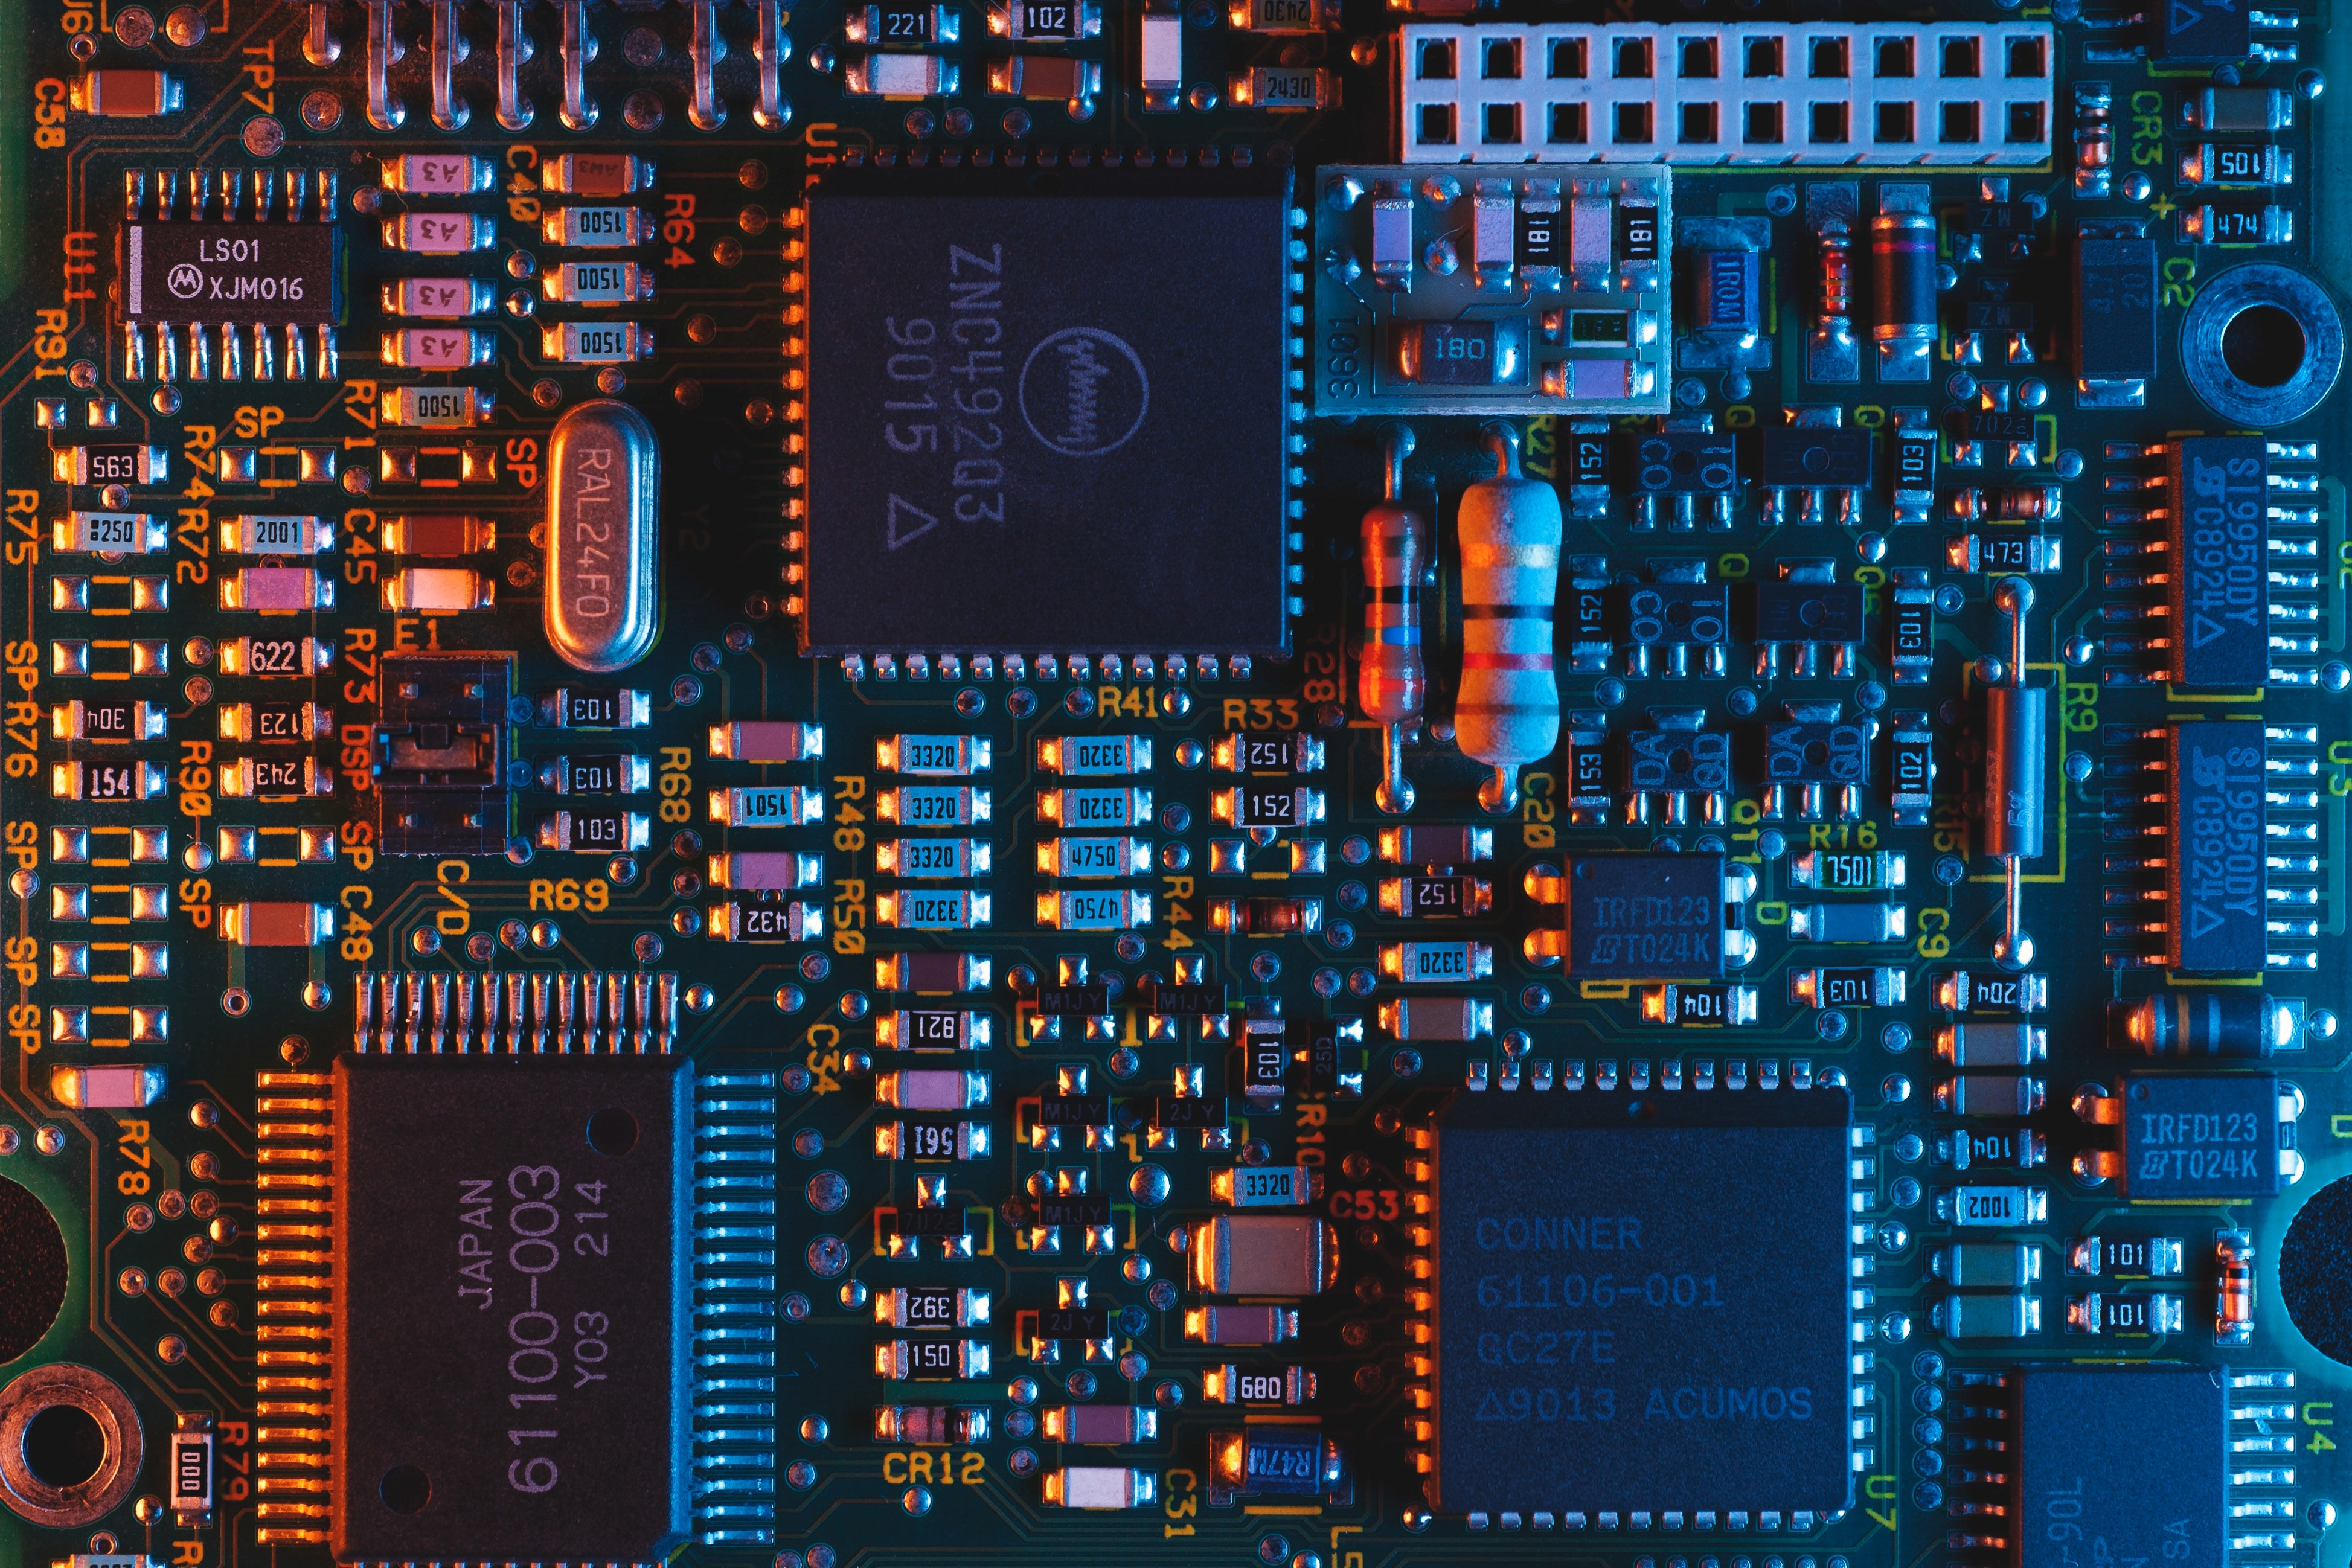
\includegraphics[width=0.9\linewidth]{graphic_name1}
% 	\caption{Caption1 Reference \cite{call_tag_article}}
% \end{figure}

\end{block}


%----------------------------------------------------------------------------------------

\end{column} % End of the first column

\begin{column}{\sepwid}\end{column} % Empty spacer column


%----------------------------------------------------------------------------------------

\begin{column}{\onecolwid} % The second column
%----------------------------------------------------------------------------------------
%	MODELS
%----------------------------------------------------------------------------------------

\begin{block}{Results \& Analysis}
\vspace{0.7em}
\textbf{Costs}

% The main objective function of the Temoa model of the Illinois energy grid minimizes total system costs, which is a high priority for policymakers and taxpayers alike. The costs of each energy technology comes in three parts:

% \begin{enumerate}
%   \item Investment costs: a one-time payment of the technology. \textit{I.e. capital cost.}
%   \item Fixed costs: an annual payment for the technology, regardless of how much it operates. \textit{I.e. operations and maintenance costs.}
%   \item Variable costs: an annual payment for the technology that varies directly with the amount it operates and produces. \textit{E.g. raw material costs.}
% \end{enumerate}

When these plants continued to operate, they did so with relatively low fixed and variable costs, since the majority of the expense of nuclear power is paid upfront via the investment cost. Without GHG restrictions imposed on the model, the cost of using other sources wasn’t significant. With restrictions imposed, the model showed increased costs in the land-use required by renewable technologies.


\begin{figure}[ht] % replace 't' with 'b' to force it to be on the bottom
  \centering
  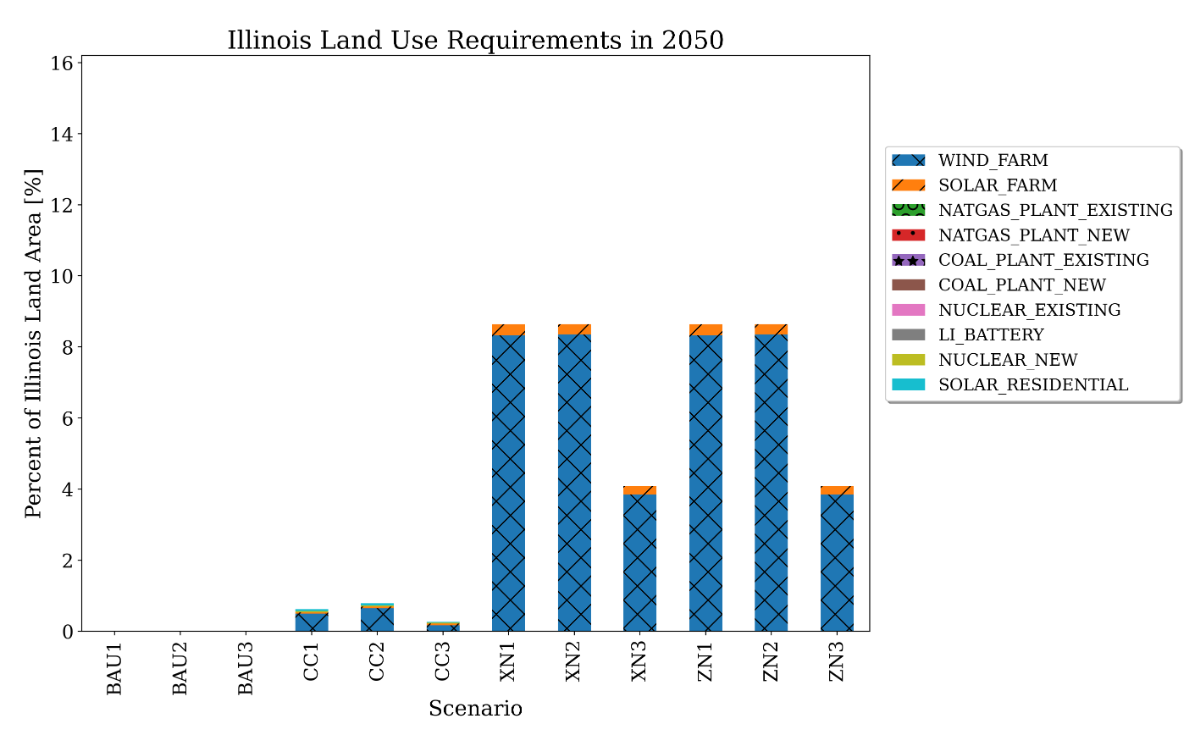
\includegraphics[scale=0.7]{land-use.png}
  \caption{Percentage of land use required for each scenario in the Dotson et al. model \cite{dotson}.}
  \label{fig:landuse}
\end{figure}

Figure \ref{fig:landuse} shows the massive increase in Illinois' land area that would be required to produce adequate levels of clean energy in the zero nuclear situation. Further, the land most suitable for such renewable implementation (specifically, solar-PV), happens to coincide with the regions used for 15\% and 14\% of corn and soybean production, respectively \cite{schleusener}.


% Example table 
% \begin{table}[]
% 	\label{tab:table_label}
% 	\caption{Table caption with citation \cite{call_tag_article}}
% 	\begin{tabular}{|l|l|l|l|}
% 	\hline
% 	Header1 &  Header2 [Units]  &  Header3 [Units]  &  Header3 [Units]   \\ \hline
% 	Item 1     & 100 & 2.5  & 2.5\\ \hline
% 	Iten 2      & 100 & 2.5 & 2.5\\ \hline
% 	Item 3     & 100 & 2.5  & 2.5\\ \hline
% 	\end{tabular}
% \end{table}

% In the waste repository model, the user can define the variables: 
% 	\begin{itemize}
% 		\item Variable
% 		\item Variable
% 		\item Variable 
% 		\item Variable 
% 		\item Variable
% 	\end{itemize}

\vspace{0.7em}
\textbf{Emissions}

The Clean Air Task Force report \cite{health} on the health impacts of these closures predicted that the decline in air quality would lead to 500 to 1,100 premature deaths—--using the EPA’s CO-Benefits Risk Assessment Health Impacts Screening and Mapping Tool (COBRA)---,costing a little over half of a billion dollars per year. 
\begin{figure}[ht]
  \centering
  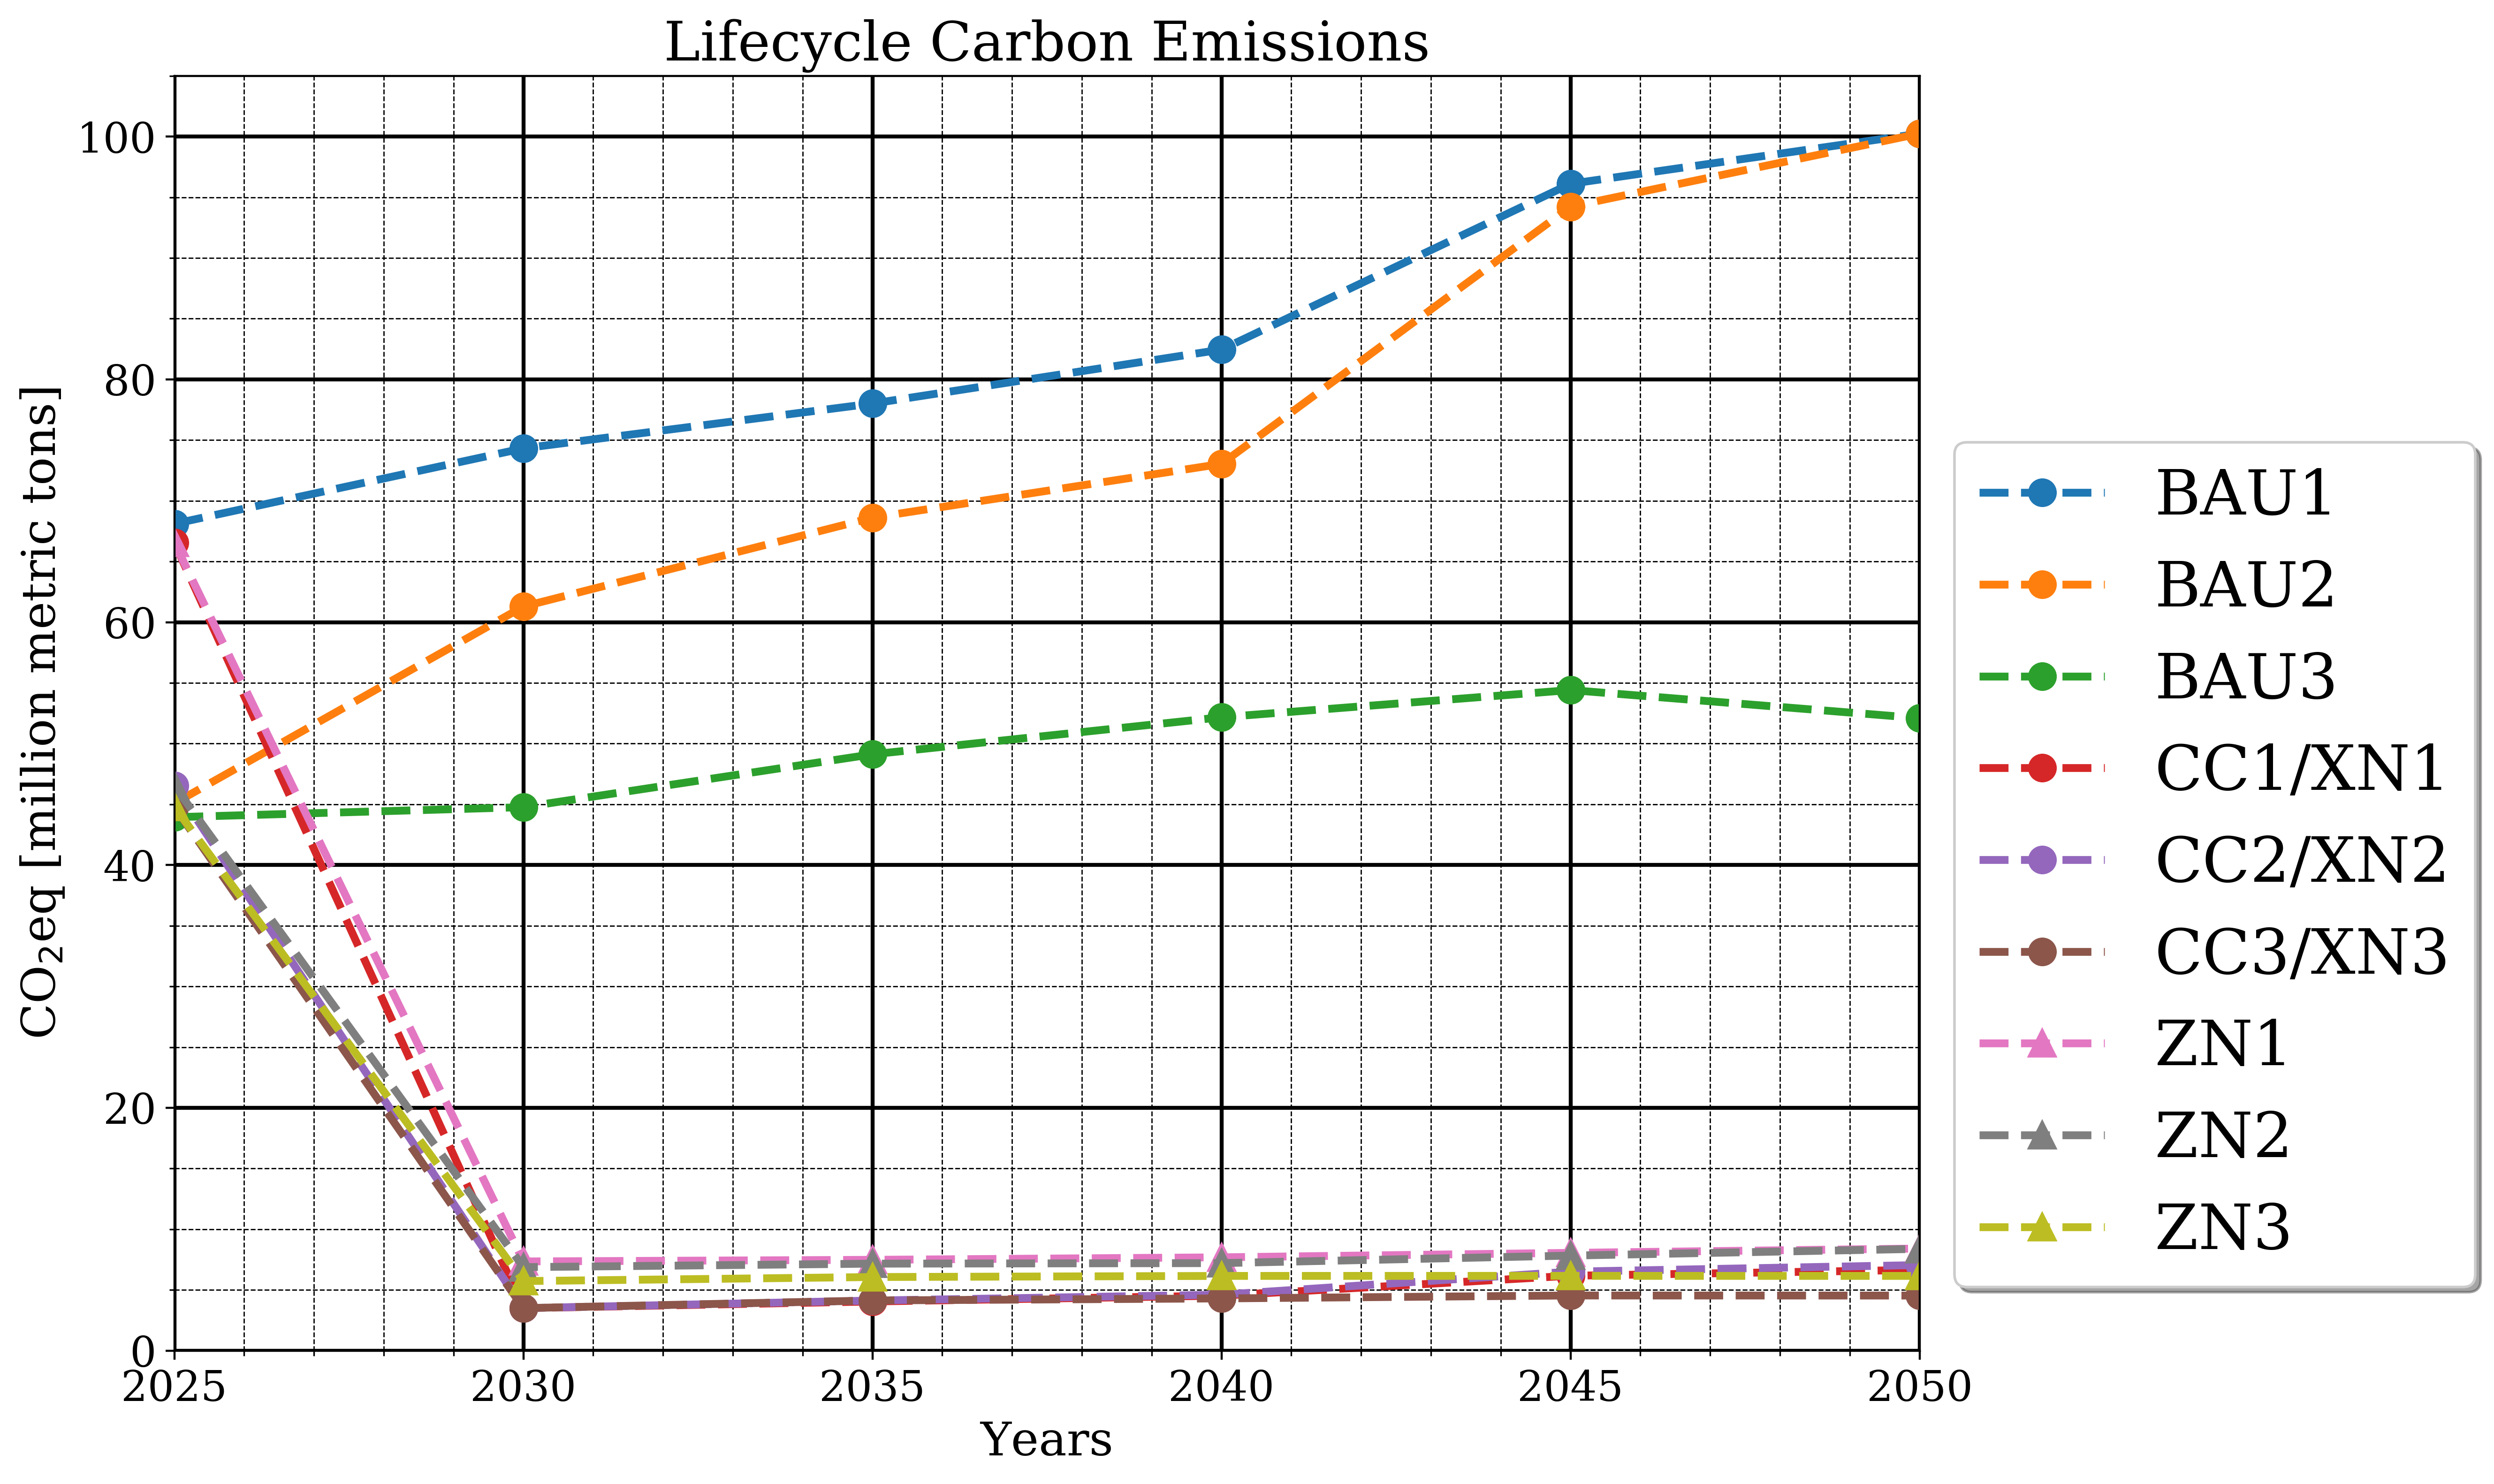
\includegraphics[scale=0.7]{co2eq_all_comparison.png}
  \caption{CO2 equivalent of lifecycle emissions for each scenario over time in the Dotson et al. model \cite{dotson}.}
  \label{fig:co2eq_time}
\end{figure}

Illinois recently joined the US Climate Alliance, committing the state to reducing their emissions to at least 26$\%$ below 2005 levels (among other promises) to track progress and accelerate technological development \cite{climate}.
% \begin{figure}[ht]
%   \centering
%   \includegraphics[scale=0.7]{co2eq_all_comparison_barplot.png}
%   \caption{Cumulative lifecycle CO2 equivalent emissions for each scenario in the Dotson et al. model \cite{dotson}.}
%   \label{fig:co2eq_cu}
% \end{figure} 

% \vspace{0.7em}
% \textbf{Third Model}

% Description with an example of a figure reference

% Figure \ref{fig:figure_label_ex1} does stuff 

% \begin{figure}
% 	\label{fig:figure_label_ex2}
% 	
\includegraphics[width=1\linewidth]{graphic_name2}
% 	\caption{Caption2 Reference \cite{call_tag_article}}
% \end{figure}

% Description 

% Equations
% \begin{align*}
% 	y = x
% \end{align*}
% Description
% \begin{align*}
% 	y = x
% \end{align*}
% Description
% \begin{align*}
% 	y = x
% \end{align*}

\end{block}


%----------------------------------------------------------------------------------------

\end{column} % End of column 2

\begin{column}{\sepwid}\end{column} % Empty spacer column

\begin{column}{\onecolwid} % The third column

\begin{block}{Conclusion}
\textbf{Something}

Description/analysis
 
Contextualization
Figure \ref{fig:figure_label_ex1} illustrates something.

Description

\begin{figure}
	\label{fig:figure_label_ex3}
	
\includegraphics[width=0.9\linewidth]{graphic_name3}
	\caption{Caption3 Reference \cite{call_tag_article}}
\end{figure}

\end{block}

% This section creates an box with an orange border and a white background
\setbeamercolor{block alerted title}{fg=black,bg=norange} % Change the alert block title colors
\setbeamercolor{block alerted body}{fg=black,bg=white} % Change the alert block body colors
\begin{alertblock}{Future Work }
	Future iterations could extend this work to take into account the effects of the recent commitments by the state to supply all of the electricity to Illionians from renewable sources by 2050.

\end{alertblock}


%----------------------------------------------------------------------------------------
%	ACKNOWLEDGEMENTS
%----------------------------------------------------------------------------------------

\setbeamercolor{block title}{fg=norange,bg=white} % Change the block title color

\begin{block}{Acknowledgements}
	
	The authors of this report would like to thank all of their co-authors on the “Economic and Carbon Impacts of Potential Illinois Nuclear Plant Closures” report upon which this research is based.
	
\end{block}

%----------------------------------------------------------------------------------------
%	CONTACT INFORMATION
%----------------------------------------------------------------------------------------

\setbeamercolor{block alerted title}{fg=white,bg=dblue} % Change the alert block title colors
\setbeamercolor{block alerted body}{fg=black,bg=white} % Change the alert block body colors

\begin{alertblock}{Contact Information}
	\setbeamercolor{block title}{fg=norange,bg=white} % Change the block title color
	\begin{itemize}
		\item Nataly: \href{mailto:panczyk2@illinois.edu}{panczyk2@illinois.edu}
		\item Nathan: \href{mailto:nsryan2@illinois.edu}{nsryan2@illinois.edu}
	\end{itemize}
% These specific elements are optional, but you should have some method for people to contact you.	
	
\end{alertblock}

\begin{block}{References}

	{\footnotesize\bibliographystyle{abbrv} 
	\bibliography{poster}}
\end{block}


%----------------------------------------------------------------------------------------



\end{column} % End of the third column

\end{columns} % End of all the columns in the poster

\end{frame} % End of the enclosing frame

\end{document}
\begin{column}{\sepwid}\end{column} % Empty spacer column
